\section*{Dictionnaire de données}

On identifie les données utiles au système d'information à partir du recueil informel des besoins.

\begin{figure}[!h]
\begin{tabular}{l l l l l l}
%
    \textbf{mnémonique} & \textbf{desc.} & \textbf{type} & \textbf{format} & \textbf{divers} & \textbf{exemple} \\
    no-adhérent          & - & entier  & -          & séquentiel & 1 \\
    nom-adéherent        & - & texte   & 50 car.    & -          & Arthur Hugo \\
    adresse-adhérent     & - & texte   & 70 car.    & -          & 14 rue de l'Université \\
    date-naissance       & - & date    & jj/mm/aaaa & -          & 01/01/2001 \\
    lieu-naissance       & - & texte   & 70 car.    & -          & Paris 11e \\
    année-validité-carte & - & date    & jj/mm/aaaa & -          & 01/01/2001 \\
    code-livre           & - & entier  & -          & séquentie  & 1 \\
    titre-livre          & - & texte   & 50 car.    & -          & La Méthode Merise \\
    nom-éditeur	         & - & texte   & 50 car.    & -          & Ed. Org. \\
    nom-auteur           & - & texte   & 50 car.    & -          & Victor Morizea \\
    date-emprunt         & - & date    & jj/mm/aaaa & -          & 20/10/2015 \\
    nom-bibliothèque     & - & texte   & 50 car.    & -          & Nanterre Info.  \\
    emplacement-livre    & - & texte   & 50 car.    & unique     & 32-10 \\
    prix-livre 	         & - & décimal & -          & -          & 6.86 \\
    est-radié            & - & booléen & -          &            & Faux \\
%
\end{tabular}
    \caption{\label{DD} Dictionnaire de données}
\end{figure}

\newpage
\section*{Diagramme de Flux}

On identifie les flux d'information en fonction du recueil informel des besoins.

\begin{figure}[!htb]
    \begin{center}
    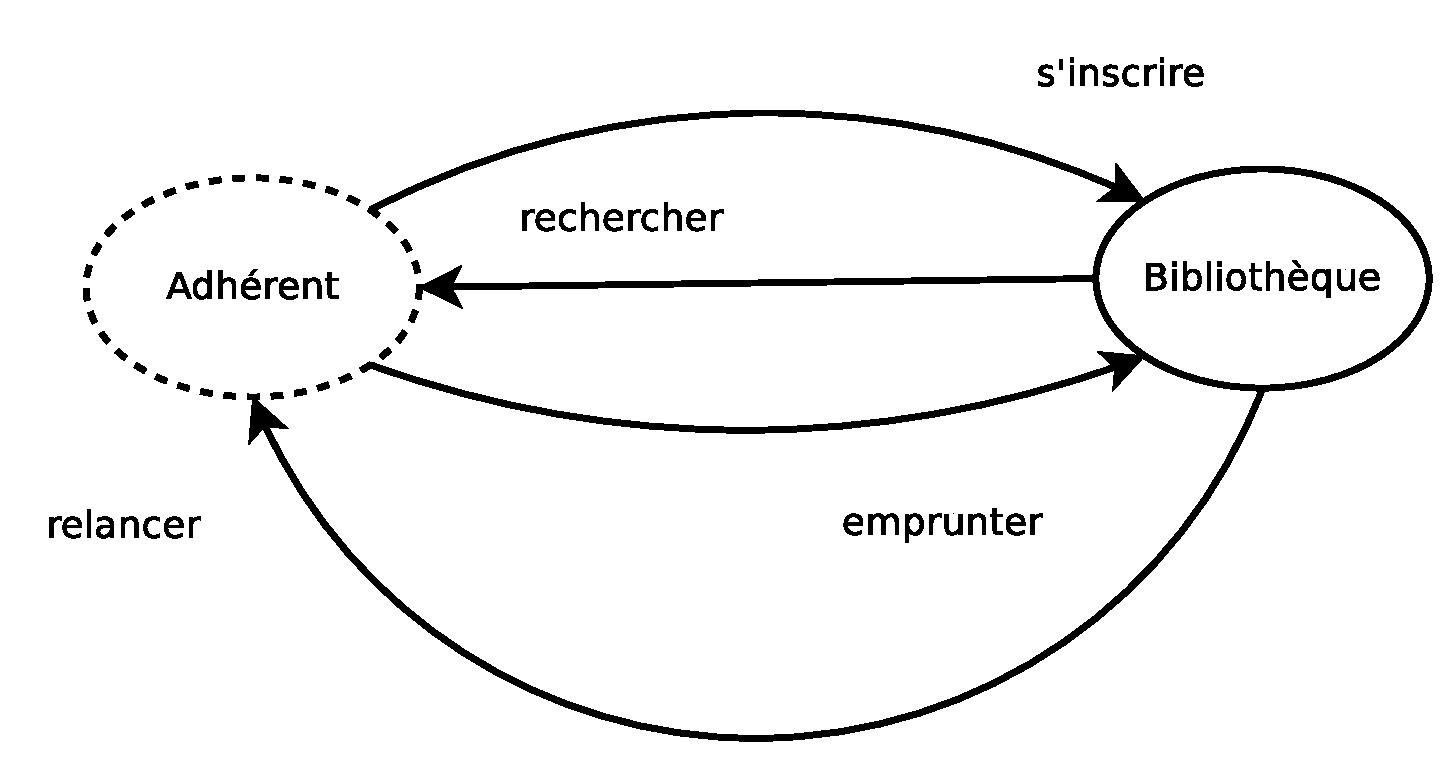
\includegraphics[width=6cm]{images/cc1_df1.eps}
    \caption{\label{cc1_df1} Diagramme de contexte}
    \end{center}
\end{figure}

\begin{figure}[!htb]
    \begin{center}
    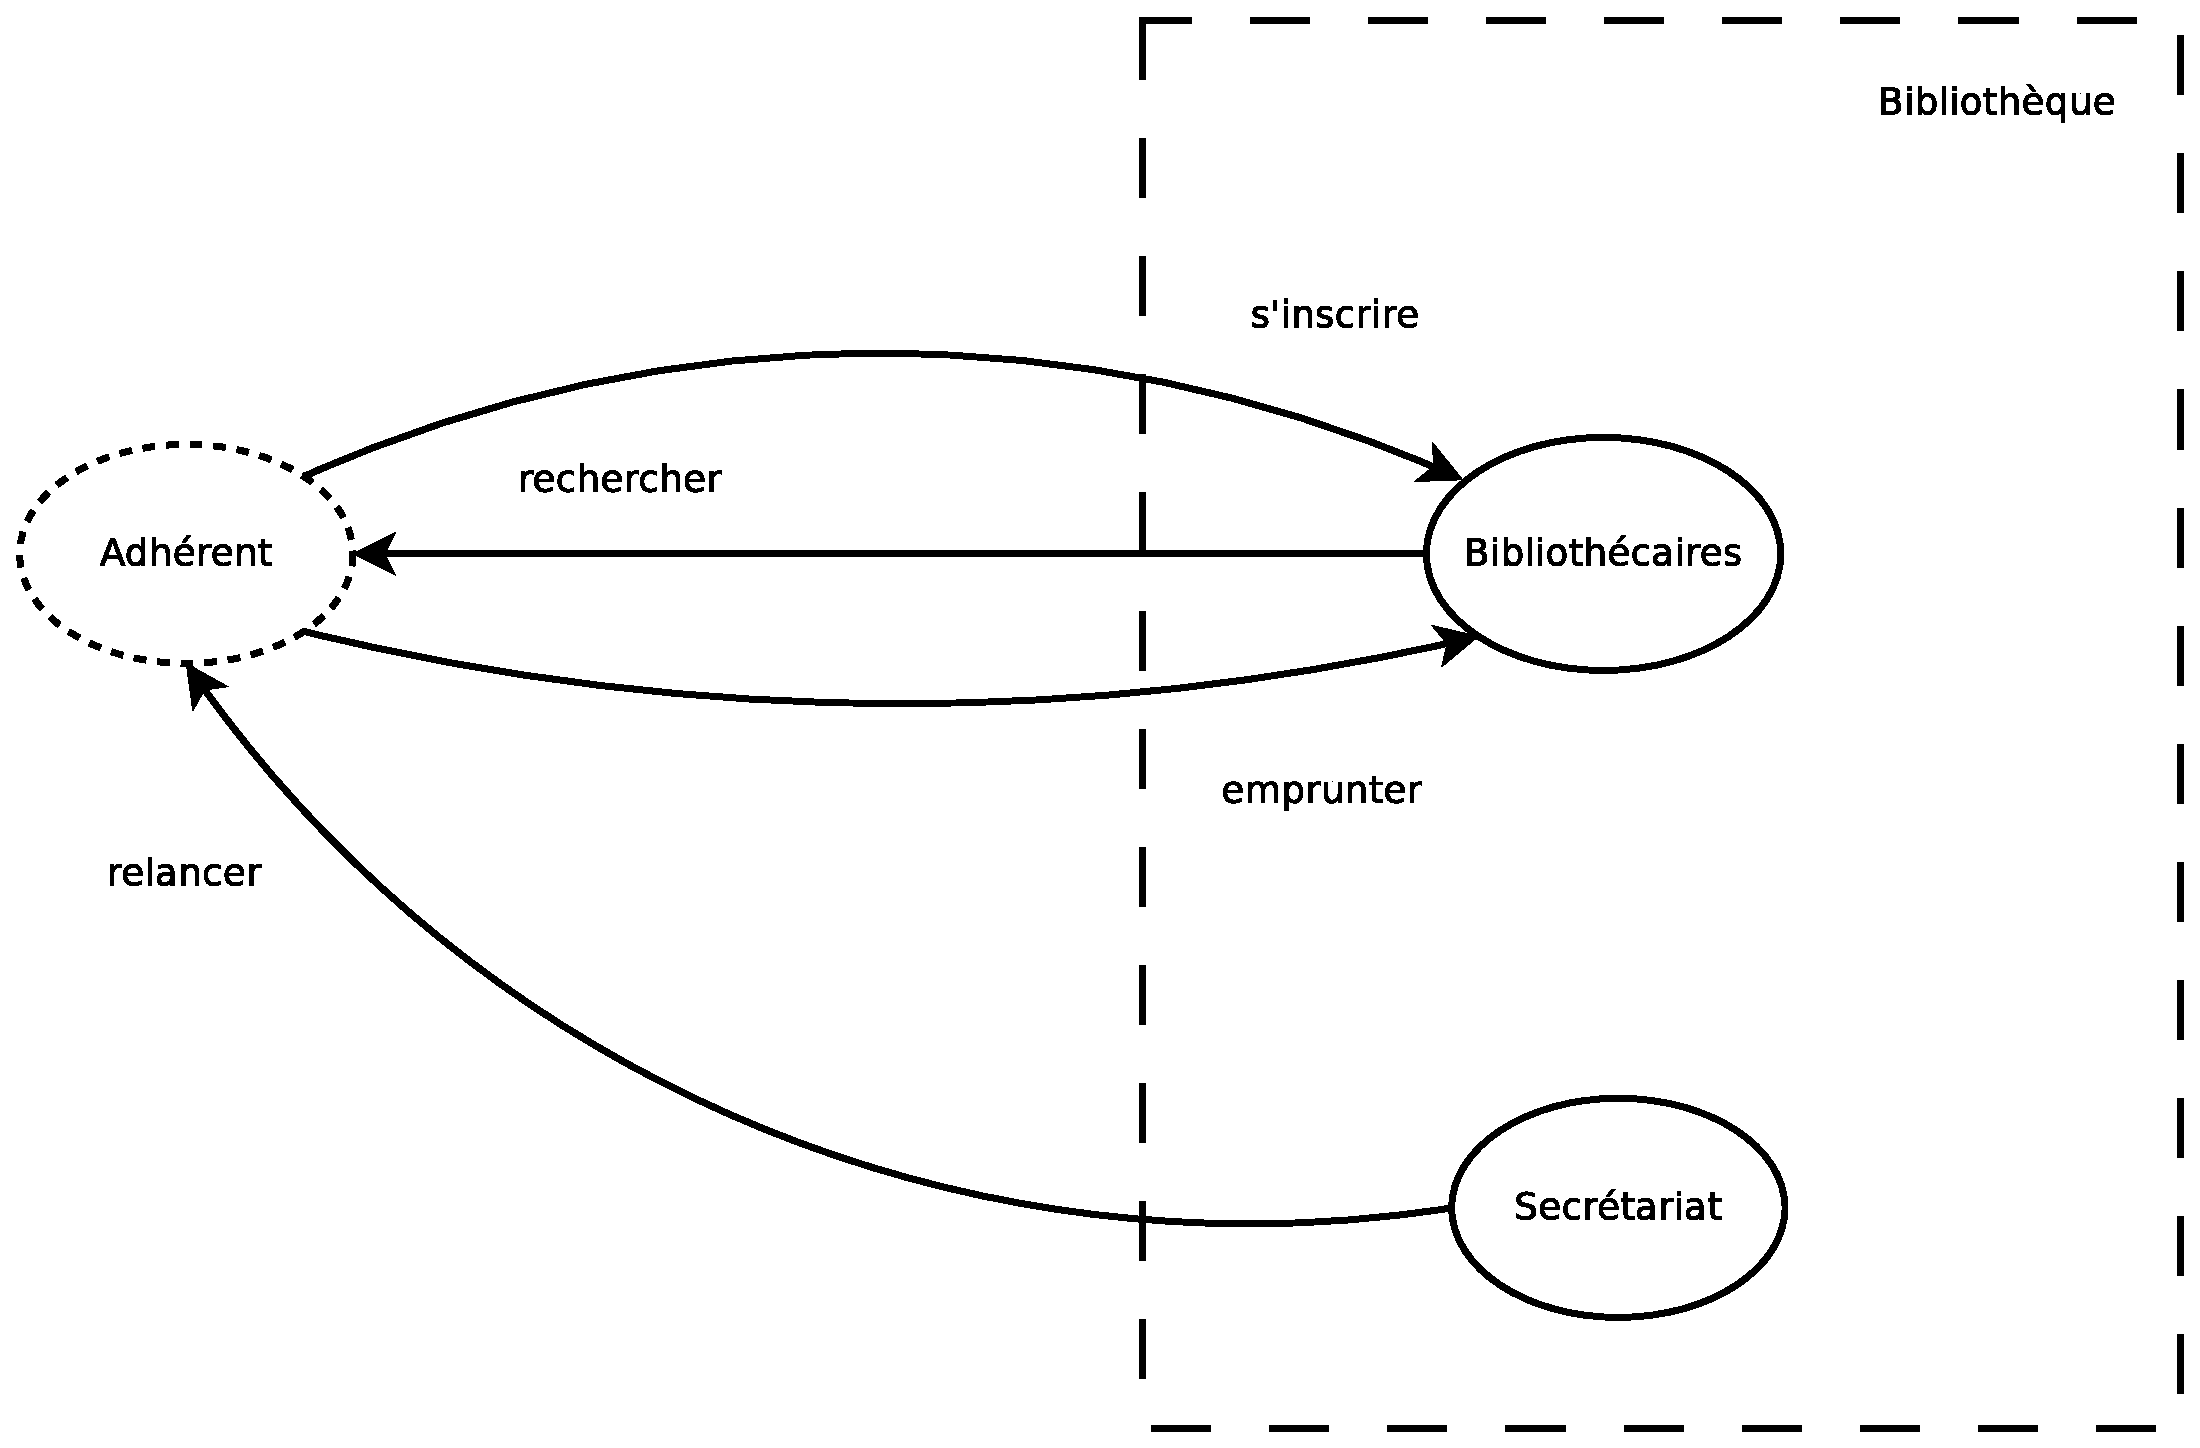
\includegraphics[width=9cm]{images/cc1_df2.eps}
    \caption{\label{cc1_df2} Diagramme des domaines d'activité}
    \end{center}
\end{figure}

\begin{figure}[!htb]
    \begin{center}
    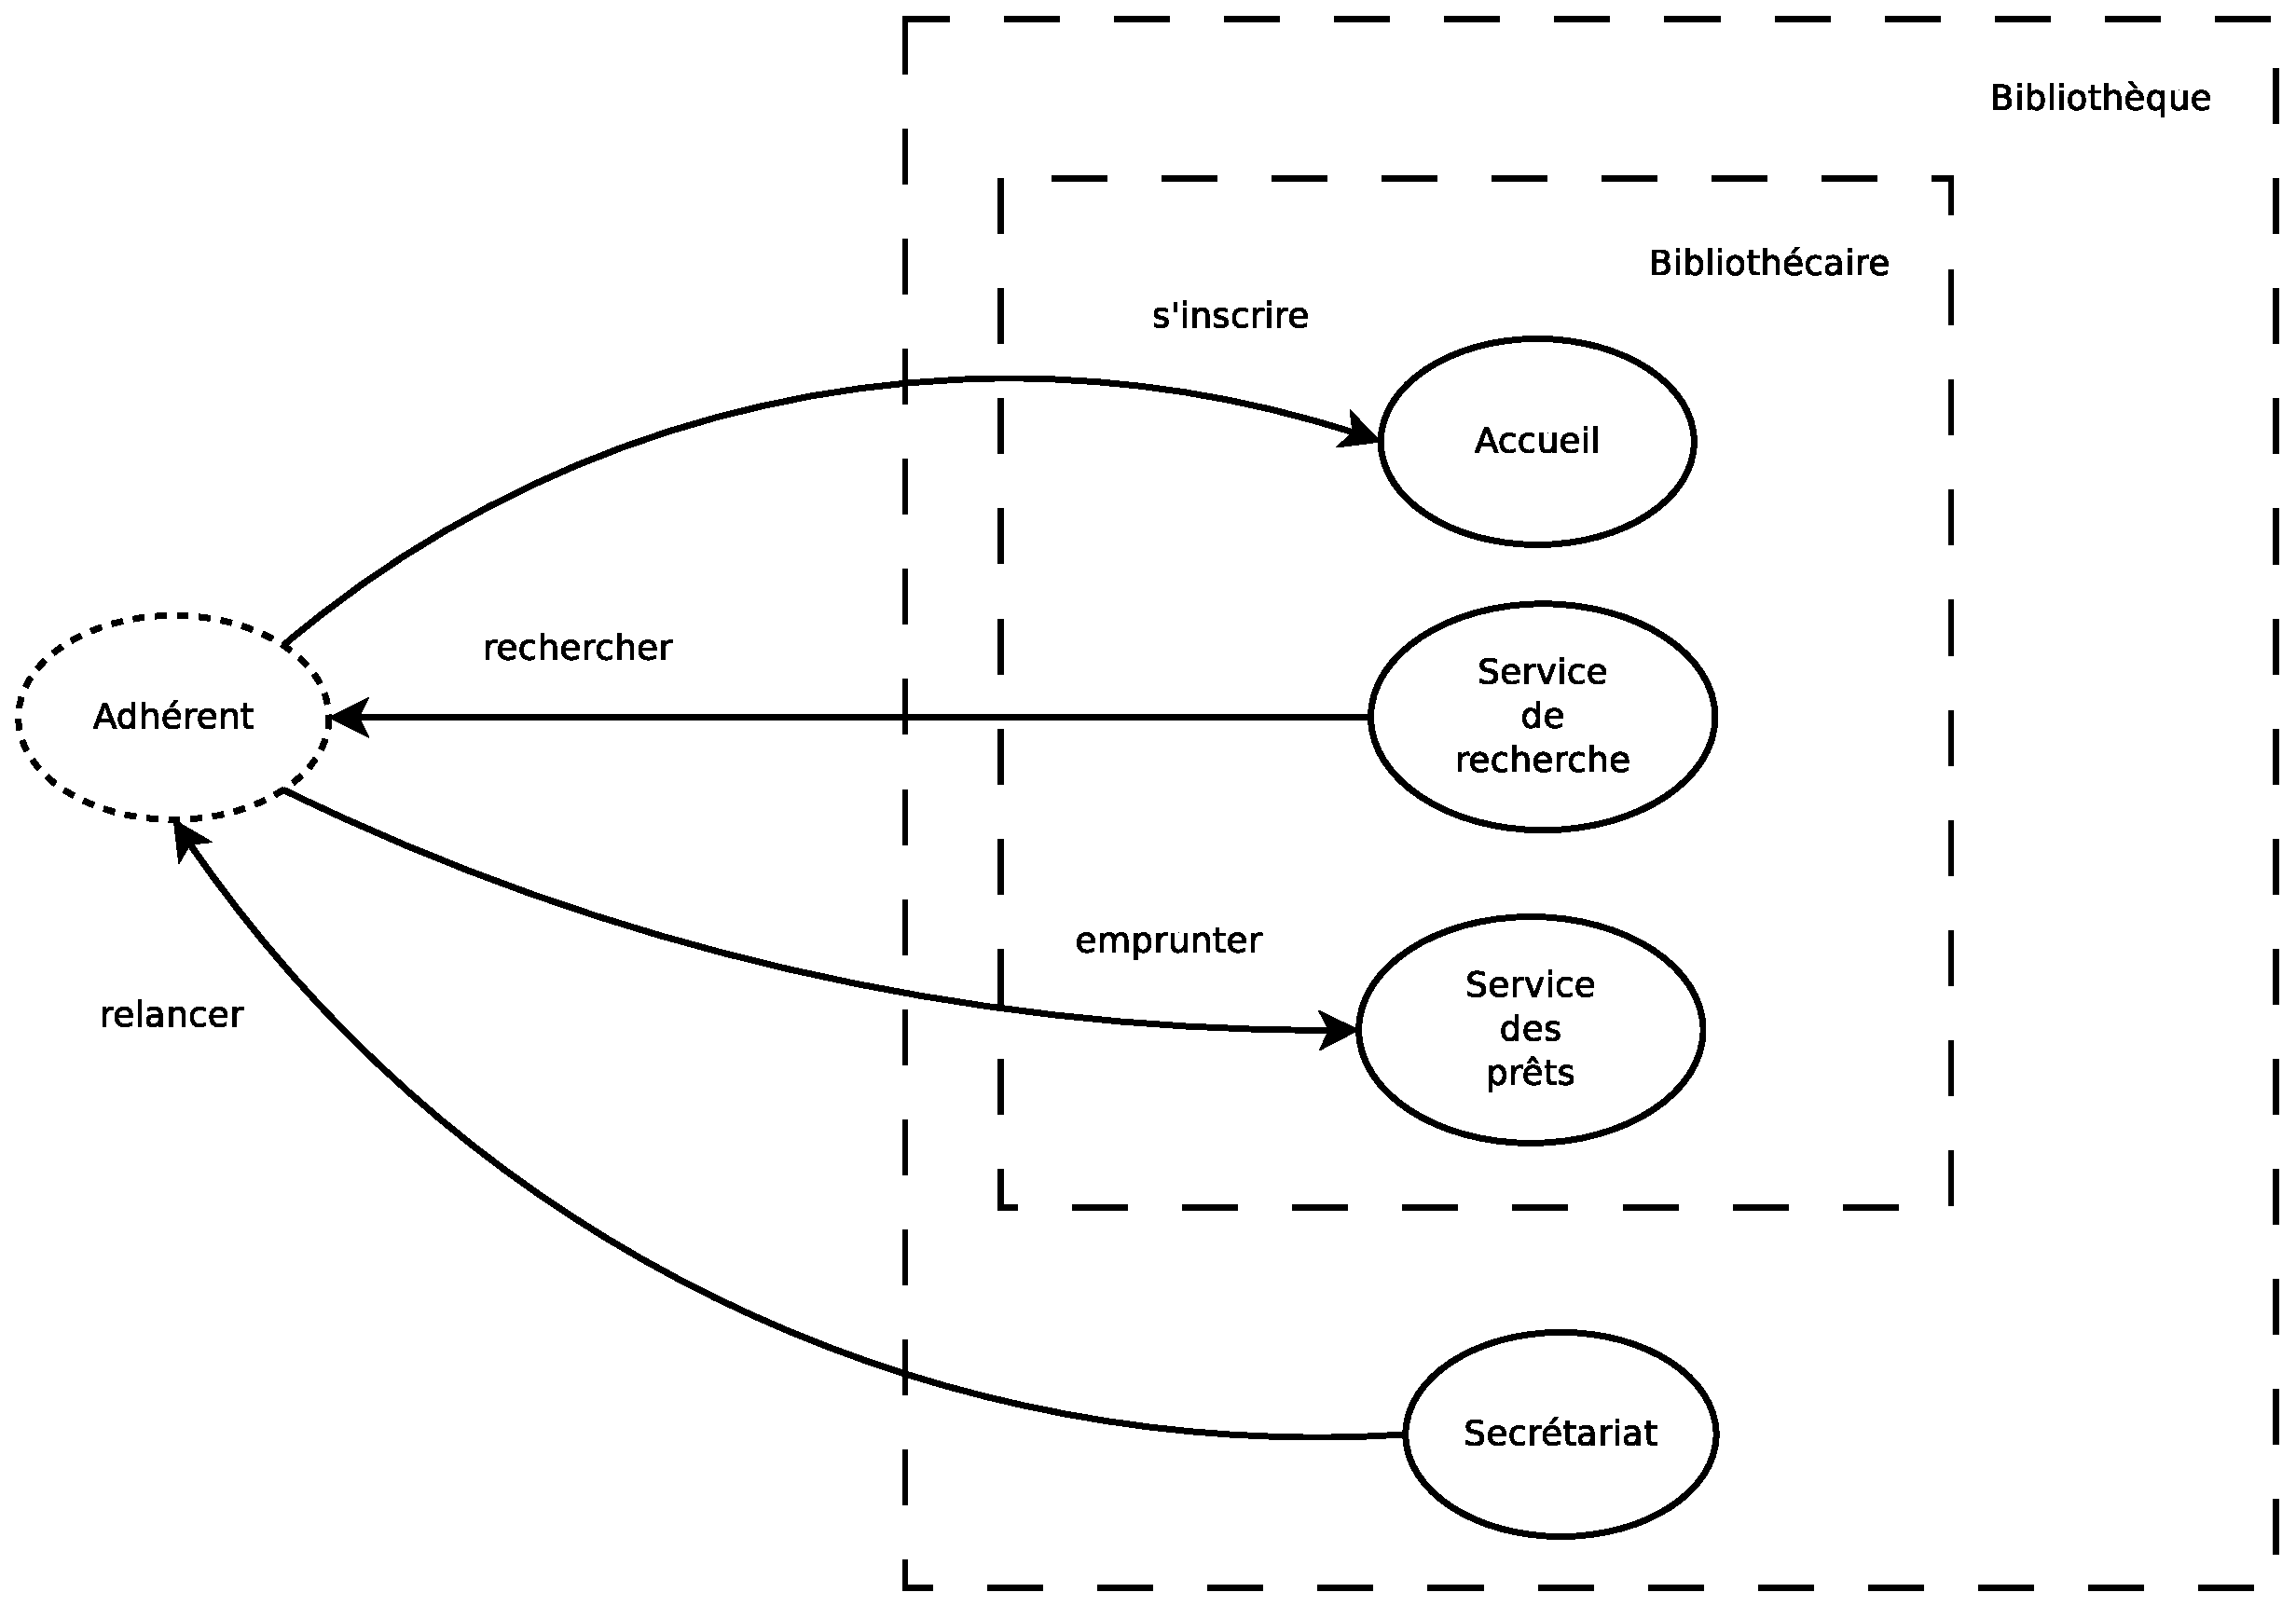
\includegraphics[width=9cm]{images/cc1_df3.eps}
    \caption{\label{cc1_df3} Diagramme de flux}
    \end{center}
\end{figure}

\section*{Matrice des Flux}

À faire à partir du diagramme de flux.

\newpage
\section*{Modèle Concptuel de Communication}

Pour chaque flux d'information du diagramme de flux, on détaille les messages échangés.

\begin{figure}[!htb]
    \begin{center}
    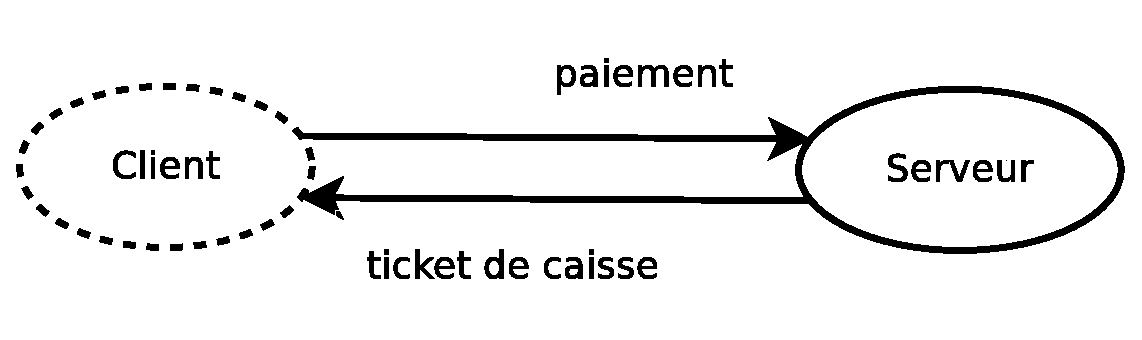
\includegraphics[width=6cm]{images/cc1_mcc1.eps}
    \caption{\label{cc1_mcc1} s'inscrire}
    \end{center}
\end{figure}

\begin{figure}[!htb]
    \begin{center}
    \includegraphics[width=6cm]{images/cc1_mcc2.eps}
    \caption{\label{cc1_mcc2} rechercher}
    \end{center}
\end{figure}

\begin{figure}[!htb]
    \begin{center}
    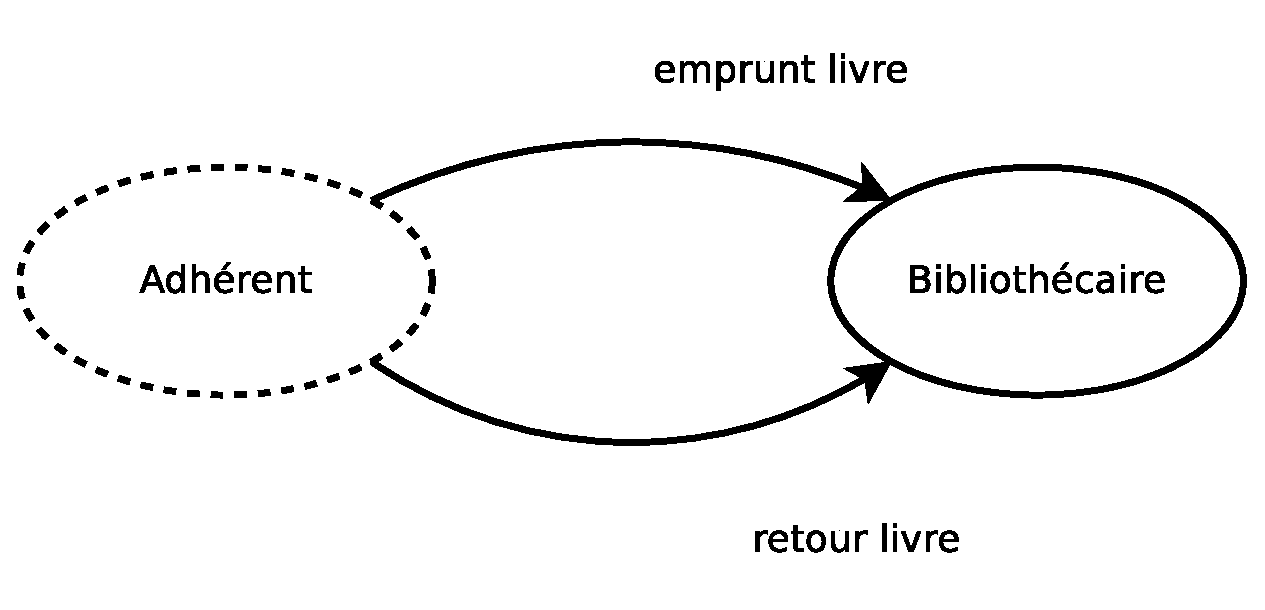
\includegraphics[width=6cm]{images/cc1_mcc3.eps}
    \caption{\label{cc1_mcc3} emprunter}
    \end{center}
\end{figure}

\begin{figure}[!htb]
    \begin{center}
    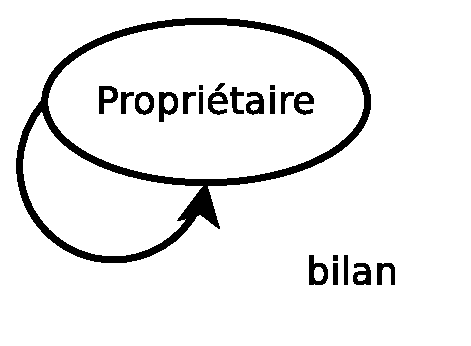
\includegraphics[width=7cm]{images/cc1_mcc4.eps}
    \caption{\label{cc1_mcc4} relancer}
    \end{center}
\end{figure}

\newpage
\section*{Modèle Concptuel de Communication détaillé}

On place affecte maintenant chaque donnée du dictionnaire de données dans le message qui la contient.

\subsubsection*{demande d'inscription(Adhérent, Accueil)}
\begin{itemize}
    \item nom-adhérent
    \item adresse-adhérent
    \item date-naissance
    \item lieu-naissance
\end{itemize}

\subsubsection*{carte d'adhérent(Agent d'accueil, Adhérent)}
\begin{itemize}
    \item no-adhérent
    \item année-validité-carte
\end{itemize}

\subsubsection*{recherche livre(Adhérent, Documentaliste)}
\begin{itemize}
    \item titre-livre
    \item nom-éditeur
    \item nom-auteur
\end{itemize}

\subsubsection*{localisation(Documentaliste, Adhérent)}
\begin{itemize}
    \item nom-bibliothèqie
    \item emplacement-livre
\end{itemize}

\subsubsection*{emprunt livre(Adhérent, Bibliothécaire)}
\begin{itemize}
    \item code-livre
    \item date-emprunt
\end{itemize}

\subsubsection*{retour livre(Adhérent, Bibliothécaire)}
\begin{itemize}
    \item code-livre
\end{itemize}

\subsubsection*{courrier de rappel(Secrétaire, Adhérent)}
\begin{itemize}
    \item no-adhérent
    \item nom-adhérent
    \item titre-livre
    \item nom-bibliothèque
    \item date-emprunt
\end{itemize}

\subsubsection*{courrier de remboursement(Secrétaire, Adhérent)}
\begin{itemize}
    \item no-adhérent
    \item nom-adhérent
    \item titre-livre
    \item prix-livre
    \item nom-bibliothèque
    \item date-emprunt
\end{itemize}

\subsubsection*{remboursement(Adhérent, Secrétaire)}
\begin{itemize}
    \item code-livre
\end{itemize}

\subsubsection*{courrier radiation(Secrétaire, Adhérent)}
\begin{itemize}
    \item no-adhérent
    \item nom-adhérent
    \item titre-livre
    \item prix-livre
    \item nom-bibliothèque
    \item date-emprunt
    \item est-radié
\end{itemize}

\newpage
\section*{Modèle Conceptuel de Données}

En suivant l'ordre des messages du MCC, on place chaque donnée véhiculée par un message dans le MCD. Pour chaque donnée, on se pose la question de l'existance d'une nouvelle entité. Une fois toutes les données placées, on valide notre MCD (formes normales).

\begin{figure}[!htb]
    \begin{center}
    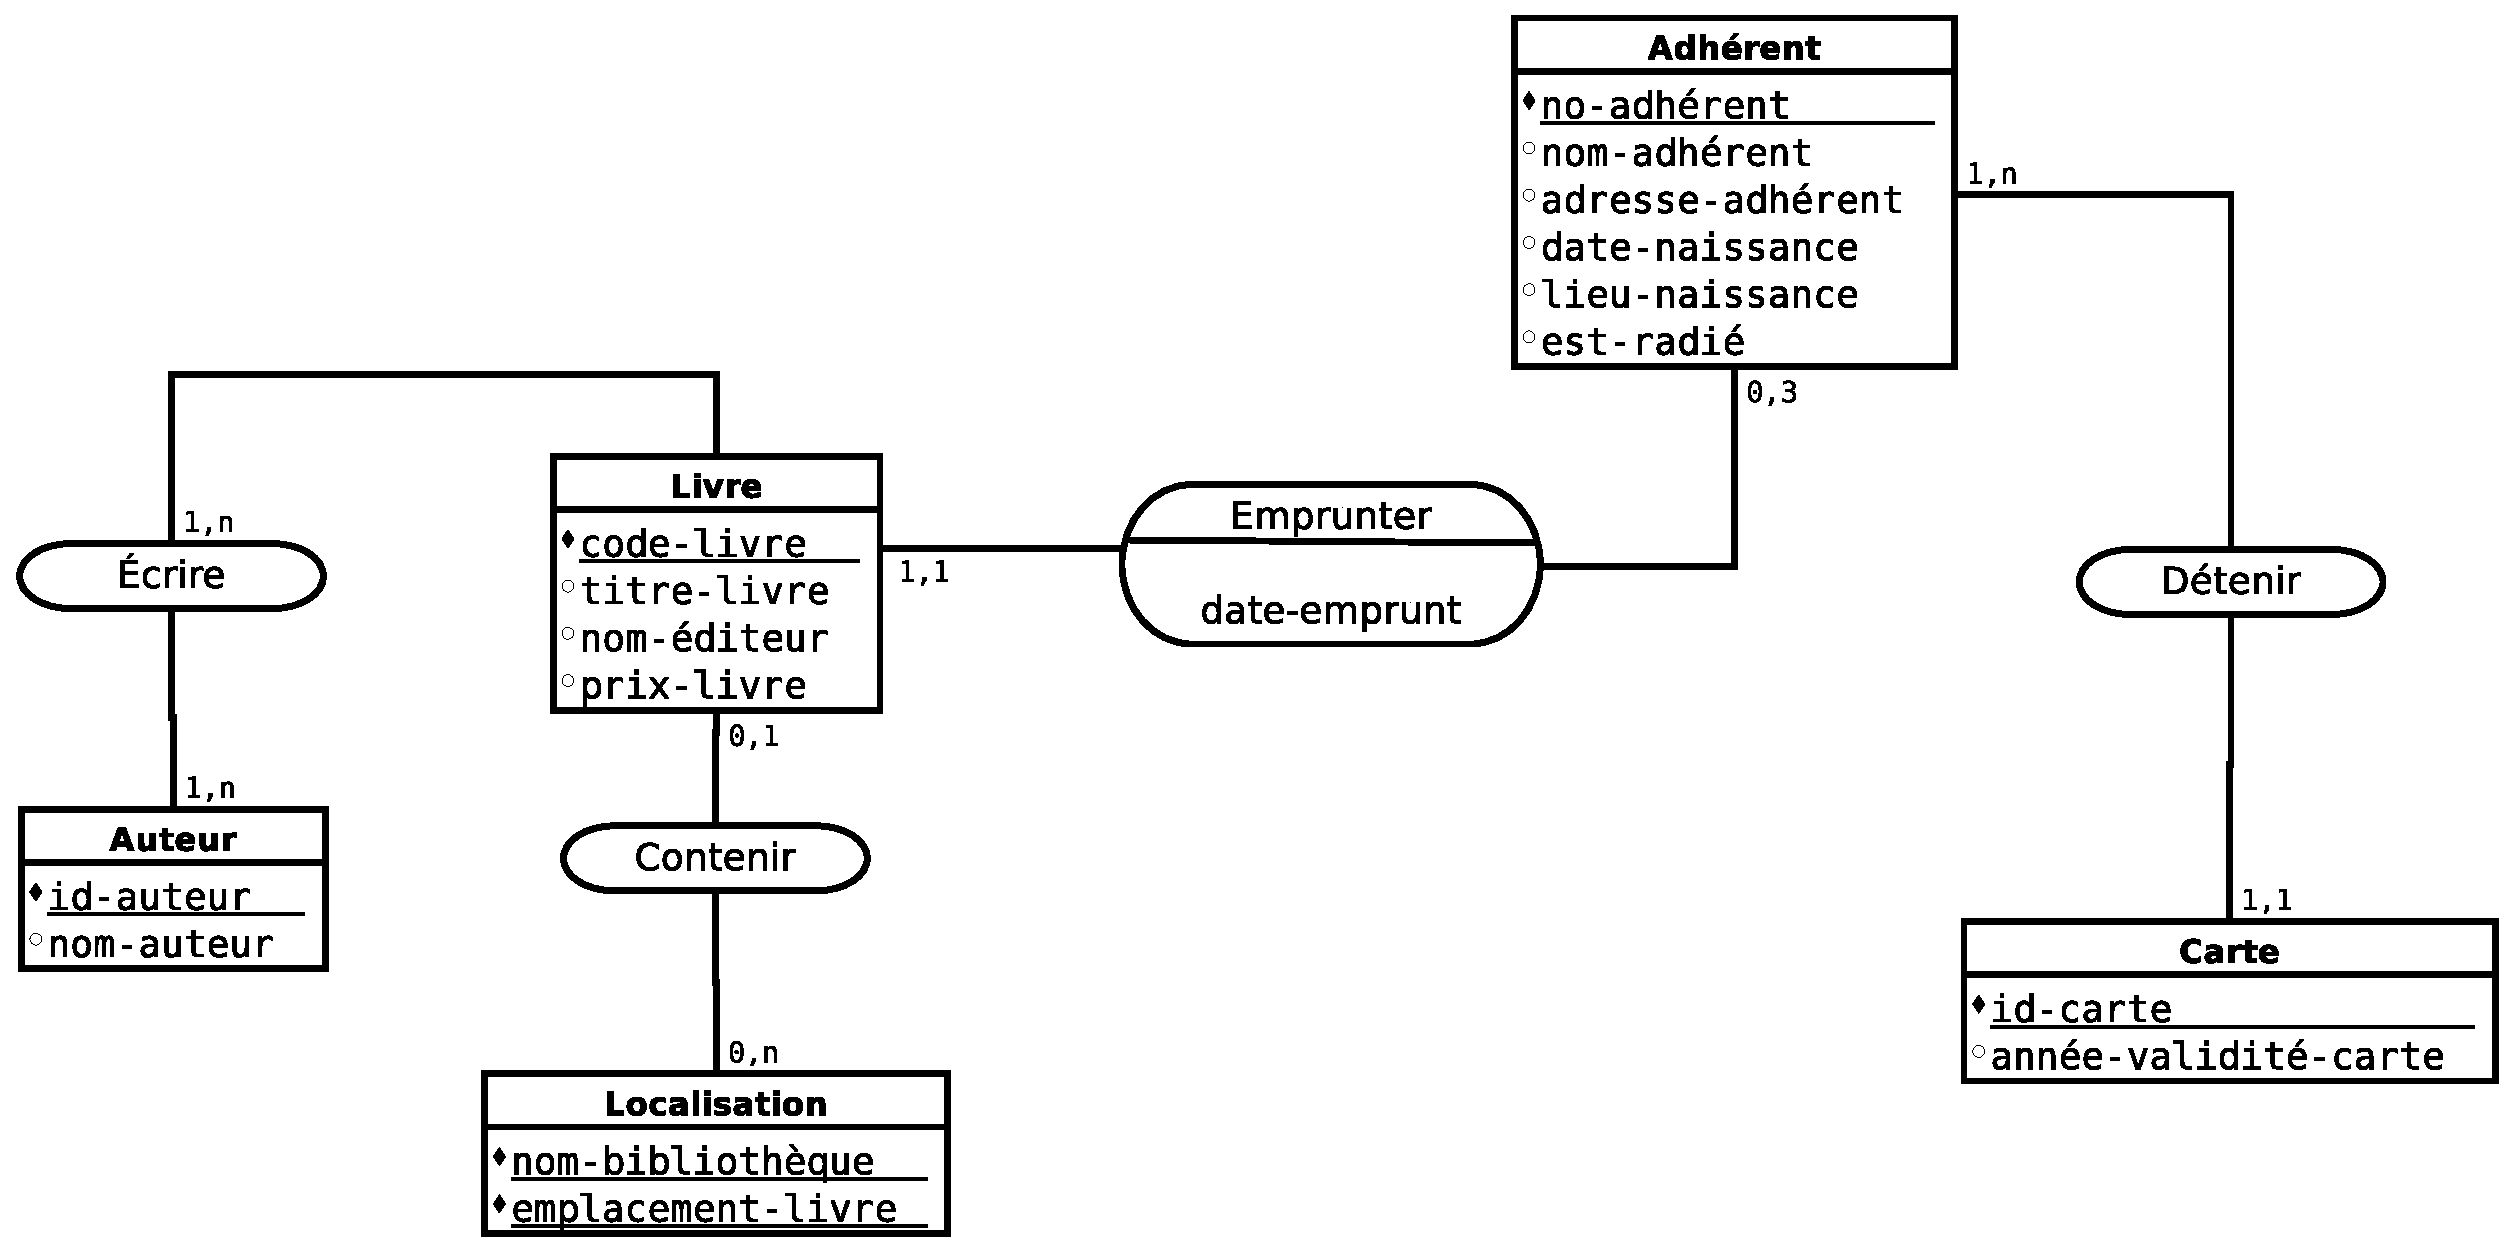
\includegraphics[width=11.5cm]{images/cc1_mcd.eps}
    \caption{\label{cc1_mcd} MCD}
    \end{center}
\end{figure}

\newpage
\section*{Modèle Conceptuel de Traitements}

Pour chaque acteur, on se demande les actions qu'il effectue sur notre système d'information.

\begin{figure}[!htb]
    \begin{center}
    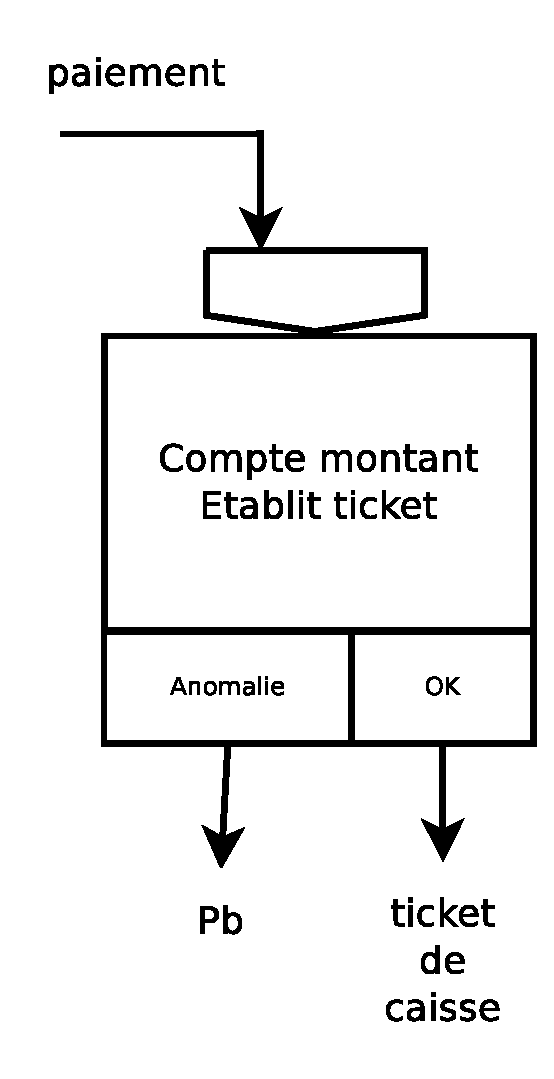
\includegraphics[height=5cm]{images/cc1_mct1.eps}
    \caption{\label{cc1_mct1} Inscription}
    \end{center}
\end{figure}

\begin{figure}[!htb]
    \begin{center}
    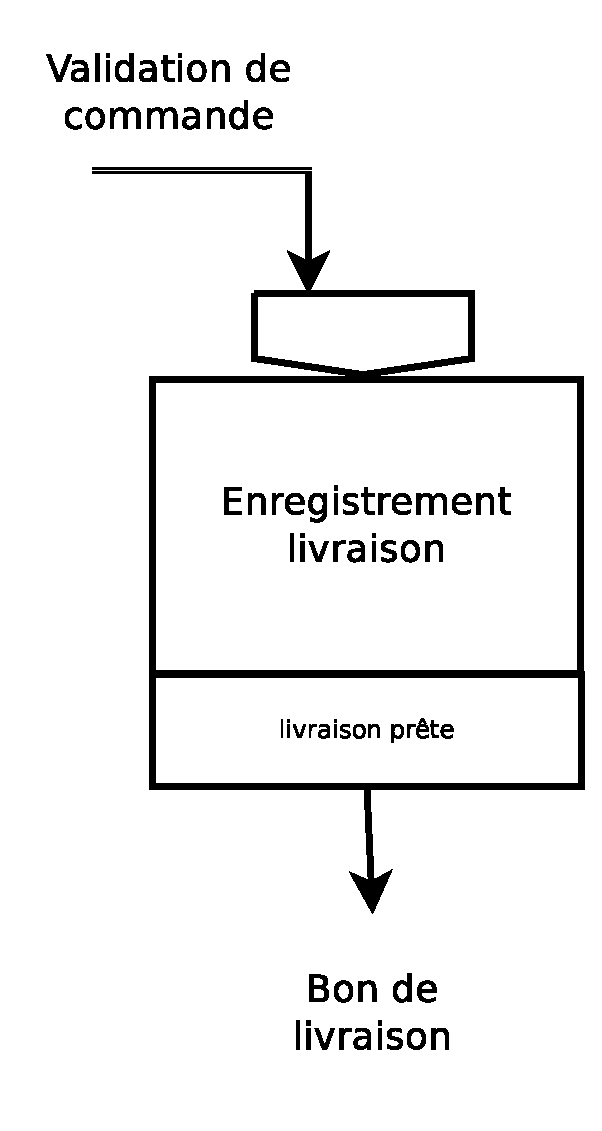
\includegraphics[height=5cm]{images/cc1_mct2.eps}
    \caption{\label{cc1_mct2} Recherche}
    \end{center}
\end{figure}

\begin{figure}[!htb]
    \begin{center}
    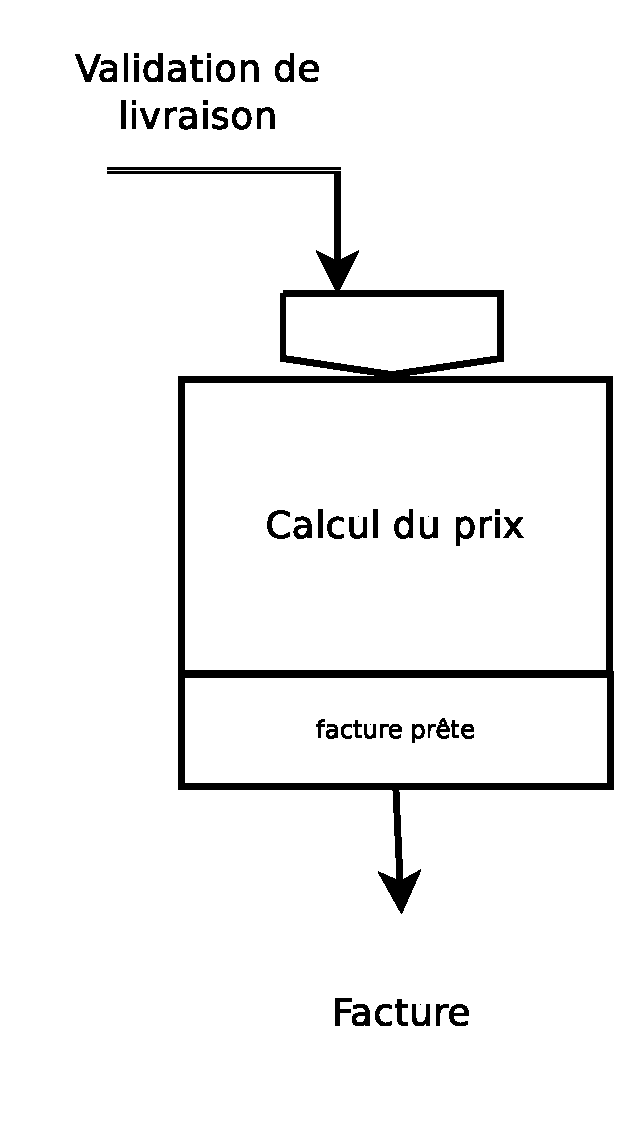
\includegraphics[height=7cm]{images/cc1_mct3.eps}
    \caption{\label{cc1_mct3} Emprunt et retour}
    \end{center}
\end{figure}

\begin{figure}[!htb]
    \begin{center}
    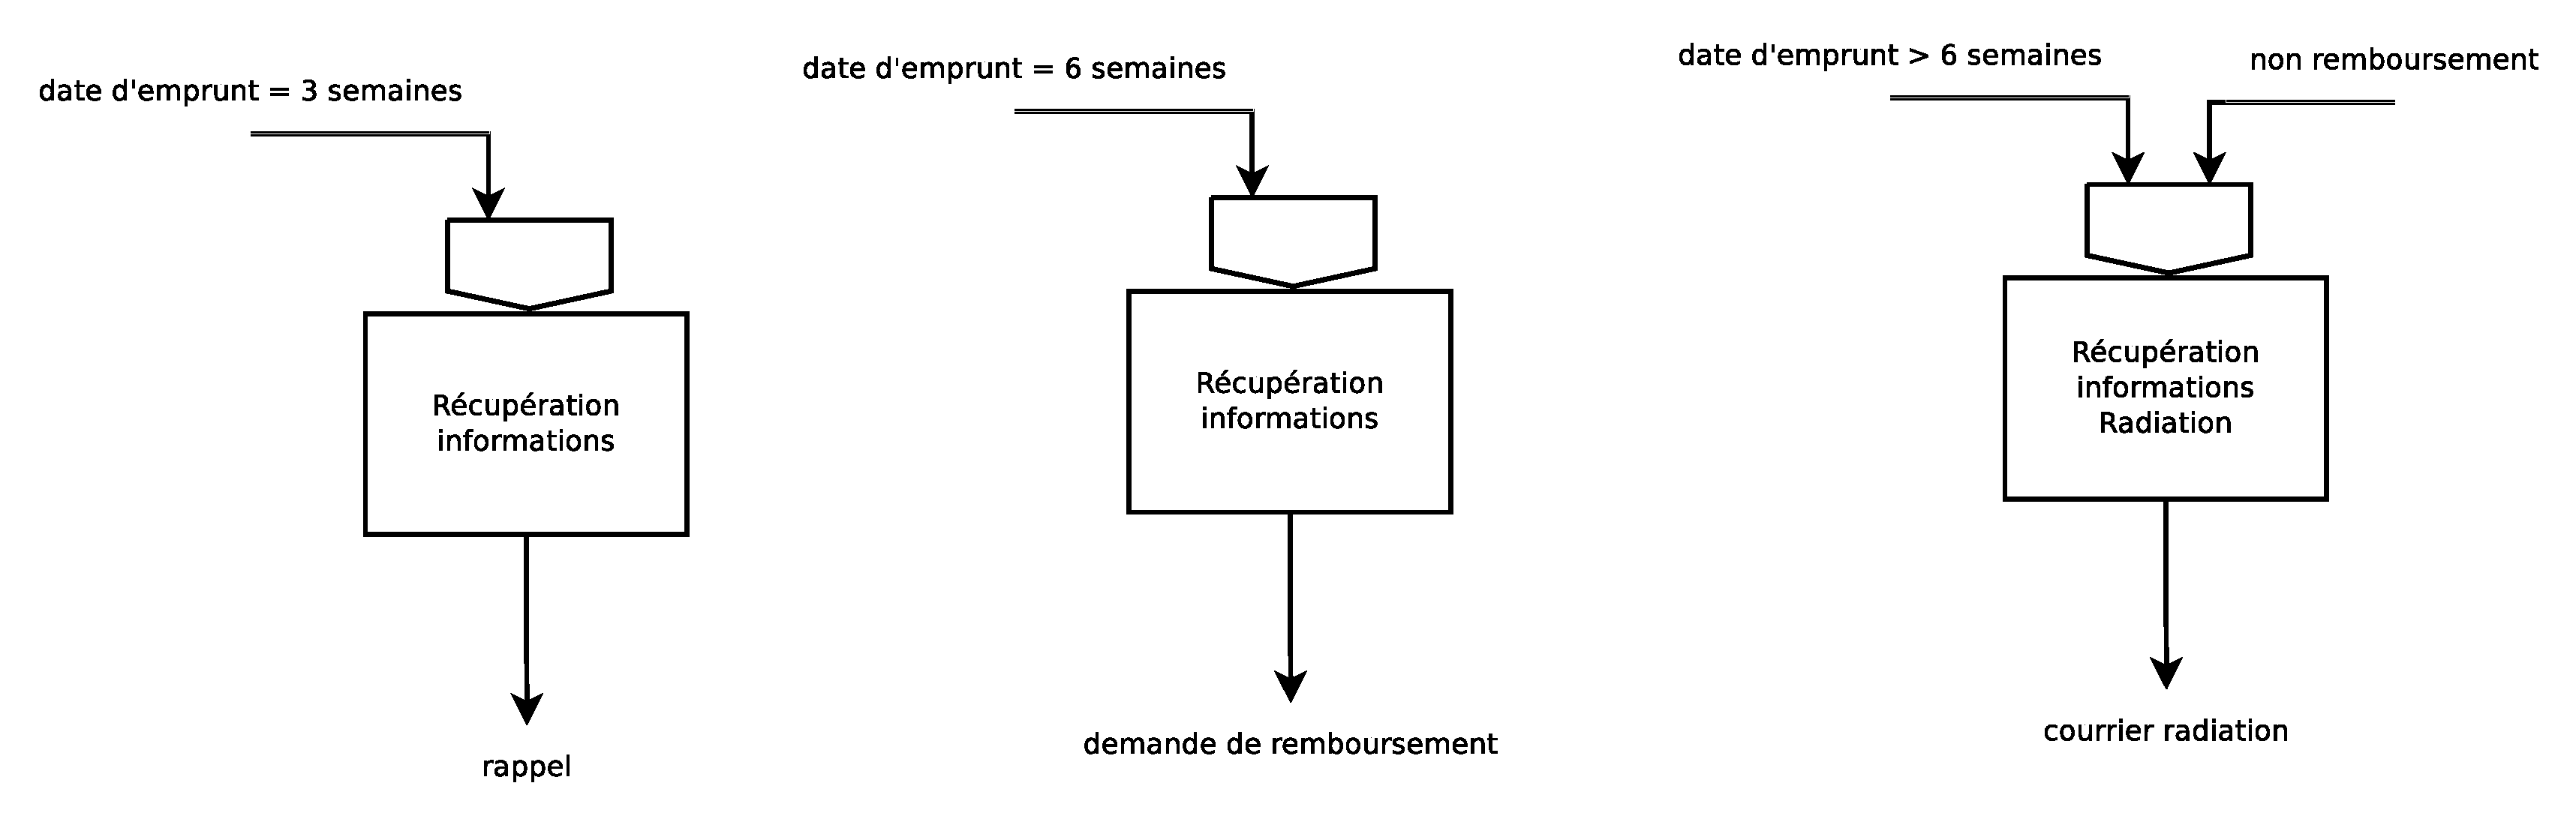
\includegraphics[height=5cm]{images/cc1_mct4.eps}
    \caption{\label{cc1_mct4} Relance et radiation}
    \end{center}
\end{figure}

\newpage
\section*{Modèle Organisationel de Traitements}

On commence par déterminer les différents postes de travail d'utilisation de notre système d'information :\\

\begin{itemize}
    \item Guichet bibliothèque
    \item Poste de recherche
    \item Poste du secrétariat
\end{itemize}

\begin{figure}[!htb]
    \begin{center}
    \includegraphics[height=6cm]{images/cc1_mot1.eps}
    \caption{\label{cc1_mot1} Inscription}
    \end{center}
\end{figure}

\begin{figure}[!htb]
    \begin{center}
    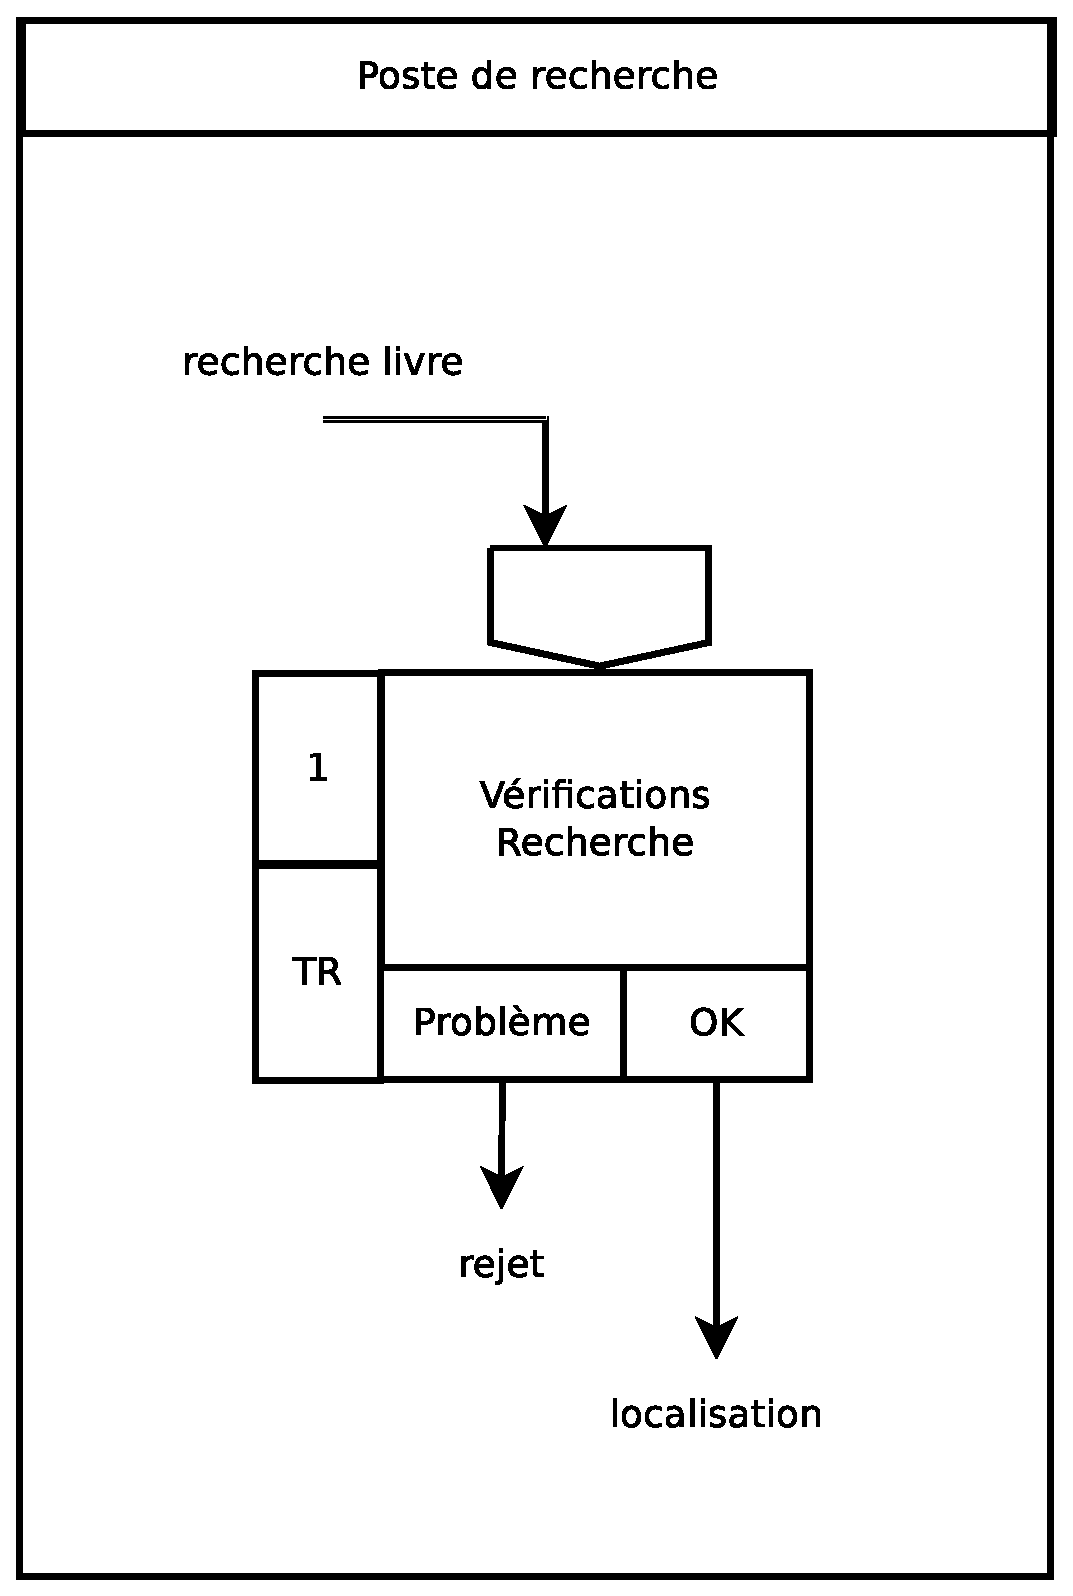
\includegraphics[height=6cm]{images/cc1_mot2.eps}
    \caption{\label{cc1_mot2} Recherche}
    \end{center}
\end{figure}

\begin{figure}[!htb]
    \begin{center}
    \includegraphics[height=12cm]{images/cc1_mot3.eps}
    \caption{\label{cc1_mot3} Emprunt et retour}
    \end{center}
\end{figure}

\begin{figure}[!htb]
    \begin{center}
    \includegraphics[height=15cm]{images/cc1_mot4.eps}
    \caption{\label{cc1_mot4} Relance et radiation}
    \end{center}
\end{figure}

\newpage
\section*{Modèle Organisationel de Données}

On commence par déterminer les différents sites de notre système d'information :\\

\begin{figure}[!h]
\begin{tabular}{l l}
%
    \textbf{Sites} & \textbf{Acteurs} \\
    Bibliothèque & Agent d'accueil \\
                 & Documentaliste \\
                 & Bibliothécaire \\
    Secrétariat  & Secrétaire \\
%
\end{tabular}
    \caption{\label{sites} Sites}
\end{figure}

On détermine ensuite les droits d'accès pour les entités et les asssociations porteuses de données :\\

\begin{figure}[!h]
\begin{tabular}{| l | c | c | c | c | c | c | c | c | c | c | c | c | c | c | c | c |}
%
   \hline
                  & \multicolumn{4}{| c |}{Agent d'accueil} & \multicolumn{4}{| c |}{Documentaliste} & \multicolumn{4}{| c |}{Bibliothécaire} & \multicolumn{4}{| c |}{Secrétaire} \\
   \hline
                  & C & R & U & D & C & R & U & D & C & R & U & D & C & R & U & D \\
   \hline
    Auteur        & - & - & - & - & X & X & X & X & - & X & - & - & - & - & - & - \\
   \hline
    Livre         & - & - & - & - & X & X & X & X & - & X & - & - & - & X & - & - \\
   \hline
    Localisation  & - & - & - & - & X & X & X & X & - & - & - & - & - & X & - & - \\
   \hline
    Adhérent      & X & X & X & X & - & - & - & - & - & X & - & - & - & X & X & X \\
   \hline
    Carte         & X & X & X & X & - & - & - & - & - & X & - & - & - & X & X & X \\ 
   \hline
    Emprunter     & - & - & - & - & - & - & - & - & X & X & X & X & - & X & - & - \\
   \hline
%
\end{tabular}
    \caption{\label{droits} Droits}
\end{figure}

On en déduit les modèles d'organisations suivants : \\

\begin{figure}[!htb]
    \begin{center}
    \includegraphics[width=11.5cm]{images/cc1_mod1.eps}
    \caption{\label{cc1_mod1} MOD Bibliothèque}
    \end{center}
\end{figure}

\begin{figure}[!htb]
    \begin{center}
    \includegraphics[width=11.5cm]{images/cc1_mod2.eps}
    \caption{\label{cc1_mod2} MOD Secrétariat}
    \end{center}
\end{figure}

